\section{The COMPSs Programming Model}
\label{sec:compss}
COMP Superscalar \cite{compss} (and, from now on, COMPSs) is a framework aimed to ease the development of applications for distributed infrastructures. A COMPSs application is typically a normal, sequential application with some special annotations and a few extra function calls in the code.\\
\\
COMPSs applications can be written in Java, C/C++, and in Python (both 2 and 3). The Python framework is called PyCOMPSs \cite{pycompss}. All the examples and real-world usages in this project will be developed in the PyCOMPSs framework and in the Python language. However, this does not mean that all the features discussed and developed in this project are only available for PyCOMPSs. In fact, given how COMPSs is designed, the implementation of a feature for PyCOMPSs usually implies to implicitly implement it for any programming language.

\subsection{COMPSs Components}
\label{subsec:compss_components}
COMPSs is designed, developed, and deployed in a modular way. This gives some advantages:
\begin{itemize} 
\item Easier isolation of features
\item Partial COMPSs installations are possible (e.g: install COMPSs without PyCOMPSs)
\item Components can be individually replaced, leading to faster deployments
\end{itemize}
An overview of the main COMPSs components can be found in figure \ref{fig:compss_modules}. These components are also modularized, as seen in figures \ref{fig:runtime_modules} and \ref{fig:pycompss_modules}.
\begin{figure}
\centering
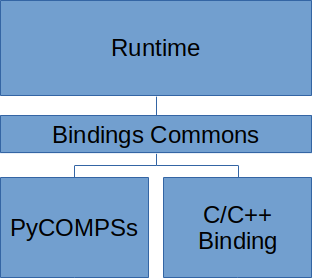
\includegraphics{figures/compss_modules.png}
\caption{Overview of the main COMPSs components. A line between two modules means that they share messages and communications between them}
\label{fig:compss_modules}
\end{figure}

%TODO: Ask Francesc help with this one
\begin{figure}
\centering

\includegraphics{figures/pending.jpg}
\caption{Overview of the main Runtime components. A line between two modules means that they share messages and communications between them}
\label{fig:runtime_modules}
\end{figure}

\begin{figure}
\centering
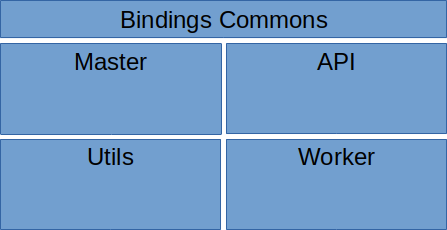
\includegraphics{figures/pycompss_modules.png}
\caption{Overview of the main PyCOMPSs components. A line between two modules means that they share messages and communications between them}
\label{fig:pycompss_modules}
\end{figure}

However, this design choice also brings some unwanted issues. The main issue is isolation and concentration of knowledge of some parts in some developers, which leads to unnecessary code replication, lack of coherence of design and implementation choices between different modules, partial feature implementations (e.g: a feature that is only available in PyCOMPSs because it was developed by someone who did not know how to implement it in the runtime), and many other things. All these issues will be adressed and referred to in this document, as they appear and play an important role in our own design choices and implementations.

%TODO
\subsection{Runtime Structure}
\label{subsec:runtime_structure}

\subsection{PyCOMPSs Structure}
\label{subsec:pycompss_structure}


\subsection{Usability vs Performance}
\label{subsec:compss_ux_vs_perf}
COMPSs has two goals: to give the not-so-expert user an easy way to make their sequential applications run in distributed environments, and to do it as efficiently as possible. Many improvements in the COMPSs framework are aimed to improve only one of these two aspects. For example, any improvement in the communication library may improve the performance of the user application, but the user will still face the same limitations and problems when using COMPSs. Adding an automatic return completion, in case the user forgot to annotate the return value of some task, may save the user a lot of debugging time, but it will have no impact in the performance of the user application.\\
\\
COMPSs is developed and mantained by a research team in a research center, so it may be natural to think that most of the efforts and improvements are aimed to test and develop methods, models, and algorithms that improve performance, memory usage, minimize network transfers and so on. However, COMPSs is also used by other research teams as a \textit{tool} for their own purposes. Some of these teams intend to run exotic, old, complicated applications in distributed environments. Also, these teams are usually composed of researchers from fields differents than computer science, so a lack of knowledge in parallel and distributed applications should be expected. The user-oriented features intend to help these research teams, making their life easier in the very complicated world of distributed computing.\\
\\
This project tries to bring something that improves COMPSs in these two directions: give something to the user that makes his life easier while making COMPSs more efficient. We do not intend to limit ourselves to give the user a way to pack some parameters in a collection. We see this feature as an opportunity to give COMPSs additional intelligence that may help to improve the performance of the framework.
